\section{Literature Review} \label{sec:lit-review}

\subsection*{QTL mapping and MAS}

The wide availability and reduced cost of molecular marker technology
has created opportunities to perform marker assisted selection of genotypes
in plant and animal breeding. Quantitative Trait Locus (QTL) mapping techniques
have proved useful for identifying markers genetically associated with genes 
conditioning agronomic phenotypes \citep{miles2008}. Using identified QTL to
support selection has grown in popularity as molecular marker data costs have 
decreased. Once a sufficient proportion of QTL-associated markers have been identified, 
the associated markers can be leveraged for making selections on a population. 
Individuals in a population genotyped for previously identified QTL-associated
markers can be selected based on the presence of desired alleles 
and/or haplotypes in a process known as Marker Assisted Selection (MAS).
MAS is usually effective on traits with a few large effect alleles with high 
heritability. However, when making selections on traits with many contributing genes
with small effect distributed widely across a genome, MAS becomes less 
effective \citep{heffner2009}.

In order to apply MAS to traits with diverse genetic architectures, it is
advisable to combine MAS on juvenile individuals and subsequent phenotypic
selection on adults with favorable MAS scores \citep{lande1990}. This process, 
known as two-stage selection, has proven effective for improving
the coefficient of selection of breeding programs while avoiding expensive phenotypic
trials for individuals with low genetic potential. While inexpensive, two-stage selection 
only utilizes those markers associated with QTL with significant effects. The present cost of
genome wide SNP assays has fallen dramatically enough that today individuals are
frequently genotyped for hundreds, thousands, or even tens of thousands of SNPs. 
Information in SNPs that are not significantly associated with a trait are lost 
when applying MAS and two-stage selection, but may still have an small effect on the
expressed phenotype and thus could provide improved predictive 
accuracy of individual's genetic value.

\subsection*{Genomic Prediction}

Unlike QTL mapping and associated MAS techniques, genomic prediction methods
attempt to predict phenotypes utilizing all available SNP marker data collected 
from a population, allowing one of many possible statistical models to predict 
the marker-trait associations in a data driven way \citep{meuwissen2001}. 
The accuracy of genomic prediction relies on an appropriate choice of a 
statistical model to capture the relationship between the genetic architecture
of a trait and the underlying marker calls in a panel of high-density marker 
data. It is likely that the best statistical model for genomic prediction is 
dependent on the genetic architecture of
the predicted trait \citep{crossa2010, gonzalez-camacho2012, 
resende2012, cleveland2012, thavamanikumar2015}.  From a mathematical perspective,
models incorporating interactions between marker features have the 
capacity to achieve higher accuracy by capturing non-additive effects.
Experimental results support this hypothesis \citep{gonzalez-camacho2012}. 
Alternative prediction methods continue to be an active area of research 
in plant and animal breeding \citep{koning2012}.

Once an accurate and predictive model of a QTL is discovered and a SNP marker
assay has been conducted on an individual, it is trivial to convert the underlying
predictions into a selection index. If the predictive model is selected 
such that it captures only additive effects, the resulting predictions can be 
considered to be an estimate of the breeding value of the assayed individual.
To differentiate breeding values estimated from genomic panels from breeding values
calculated via traditional phenotypic measurements and best linear unbiased prediction (BLUP)
models, the term genome estimated breeding value or GEBV was coined \citep{meuwissen2001}.

\subsection*{Choosing a Genomic Prediction Model}

Genomic prediction presents a distinct mathematical challenge compared to MAS.
When conducting MAS, a large number of individuals $n$ are evaluated at a
comparatively smaller number of loci $p$. In a general sense, this corresponds 
to solving an overdetermined system of linear equations. The large family of 
regression techniques that minimize a least-squares loss function are well
behaved on overdetermined systems. Genomic prediction is characterized by the opposite
scenario where $n < p$. Typically a smaller number of individuals are genotyped
at a larger number of marker loci. These problems can be solved using least squares regression,
but also require that a regularization penalty is included in the calculations in 
addition to the least-squares loss function that is used to select between 
possible solutions to the underdetermined system.

There are many forms of regularization. Perhaps the best known is L2 regularization, 
which penalizes large regression coefficients in least squares regression 
problems \citep{tibshirani1996}. Because L2 regularization penalizes the squares of the coefficients 
in the model, solutions that place a small coefficient on many available input features 
produces a lower value for the model's loss function than a model with equivalent accuracy 
that uses large coefficients on only a few input features. This results in a trained
model that tends to place a small coefficient on all available input features.  Ridge regression
is an example of an L2 regularized ordinary least squares regression. 

Another common form of regularization is L1 regularization \citep{tibshirani1996}. 
L1 regularization penalizes the sum of the regression coefficients in least 
squares regression problems. This causes solutions that set many input feature 
coefficients to zero to produce a lower total loss value than alternatives 
with equivalent prediction accuracy that utilize more input features. 
As a result, L1 regularization tends to produce solutions that set non-informative 
feature's coefficients to zero. Least absolute shrinkage and selection operator 
(LASSO) regression is an L1 regularized ordinary least squares regression. Both L1 and L2
regularization techniques can be applied to the weights of a neural network's neurons
as described in Subsection \ref{ssec:neuralnets}.

Different regularization techniques such as L1 and L2 regularization have a relationship
to the genetic architecture of the trait they being used to predict. If a trait is associated 
with many small effect markers, models incorporating L2 regularization are likely 
to perform better than unregularized models. Classical MAS traits with a small 
number of large effect markers may be best predicted by algorithms 
incorporating L1 regularization. Traits falling somewhere in between may do well 
with models incorporating a combination of L1 and L2 regularization such as
elastic net regression \citep{zou2005}.

A wide variety of regularization techniques exist. Some are broadly used and simple
to reason about like L1 and L2 regularization. Others are applicable only to certain 
classes of mathematical models such as assumed prior distributions in Bayesian
regression methods. When choosing a tool for genomic prediction, it is critical to evaluate 
the available regularization techniques with multiple prediction methods in a data-driven way.
These comparisons will ideally identify a single best model with zero or more regularization techniques 
which can be used to make accurate predictions for the traits of interest. 

\subsection*{Data Science}

As interest in using genomic prediction as a breeding tool grew, the research in 
the interdisciplinary field known as data science has increased. Data scientists 
use machine learning and statistics to make 
predictions, usually by applying ideas or techniques from a wide variety of domains 
including mathematics, statistics, and computer science. Often, a data scientist's focus is to
create a predictive model that may not be associated with an underlying generative model. 
Some view this as the distinction between data science and classical statistics 
\citep{donoho2015, breiman2001}. The rapid increase in popularity of data science
is associated with better definitions of best practices for predictive modeling
across many disciplines as well as software packages to automate the 
process of building predictive models from any data source.

Data scientists have used their experience to improve existing statistical 
models and tackle problems of immense complexity, some of which were previously 
thought to be unsolvable. Data scientists have applied neural networks to recognize 
handwritten text or generate transcripts of spoken words from real-time audio recordings \citep{lang1990}.
Data scientists compared the performance of a neural networks model to a traditional 
logistic regression model used to detect signals indicating epilepsy in electroencephalograph 
readings and found the network unanimously outperformed the existing model \citep{subasi2005}.
A complex neural network architecture was used to play seven different Atari 2600 
games using screen pixels as input and training the network to maximize a score metric 
for the game it was trained on \citep{mnih2013}. These results demonstrate that machine learning,
and neural networks in particular can be employed to solve problems or improve predictive accuracy
on large and complex datasets from a wide variety of fields.

The successes has renewed interest in the machine learning field in both
private and public sectors. Many universities now offer advanced cross-disciplinary
degrees in data science that include statistics, mathematics, and computer
science training. Genomic prediction is one of many opportunities for data scientists
to apply these tools to plant and animal breeding.

\subsection*{Neural Network Architecture} \label{ssec:neuralnets}

Neural networks are a type of model frequently employed by data scientists
for predictive modeling. Neural networks consist of layers of interconnected neurons
which map inputs to one or more outputs. Each neuron in a network can be expressed as a 
transformation of a weighted sum of $n$ inputs 

\begin{equation}
output_{lk} = \sum_{i=1}^{n} f_l(w_{lki} * x_{i} + b_{lk})
\label{eq:neuron}
\end{equation}

where $output_{lk}$ is the output from neuron $k$ in network layer $l$ having activation
function $f_l$, weights $w_{lki}$ and bias $b_{lk}$.

A neural network is a collection of neurons that map a 
length $n$ input vector $x = (x_1, ..., x_n)$ through a series of $j$ 
"hidden" layers $(l_1, ..., l_j)$. Each hidden layer consists of a variable 
number of neurons, each of which apply an associated coefficient, bias, and 
mathematical transformation to their input and forward the 
result on to every neuron in the subsequent layer forming an interconnected
network (Figure \ref{fig:simplenet}).

\ifdefined\showtablesandfigures
% A simple neuralnet with one hidden layer.

\begin{figure}[htbp]
\renewcommand{\familydefault}{\sfdefault}\normalfont
\centering

\def\layersep{2.0cm}

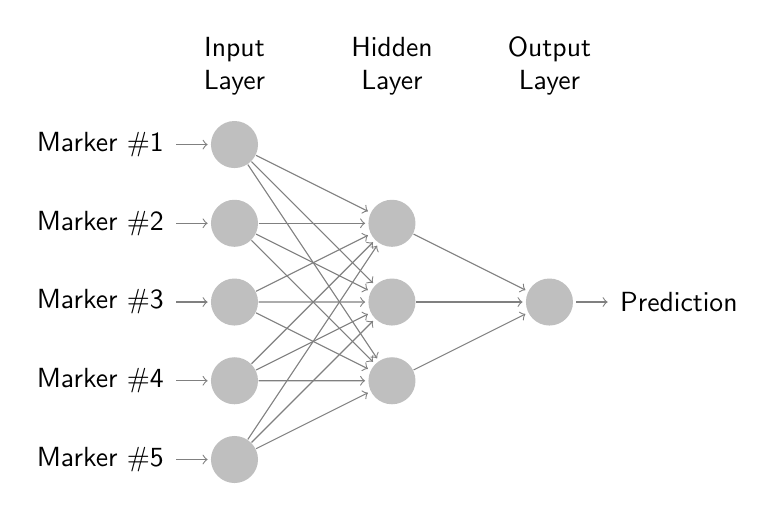
\begin{tikzpicture}[shorten >=1pt, ->, draw=black!50, node distance=\layersep]
    \tikzstyle{every pin edge}=[<-, shorten <=1pt]

    \tikzstyle{neuron}=[circle, fill=black!25,minimum size=17pt, inner sep=0pt]
    \tikzstyle{input neuron}=[neuron];
    \tikzstyle{output neuron}=[neuron];
    \tikzstyle{hidden neuron}=[neuron];

    \tikzstyle{annot}=[text width=4em, text centered]

    \foreach \name / \y in {1,...,5}
        \node[input neuron, pin=left:Marker \#\y] (I-\name) at (0,-\y) {};

    \foreach \name / \y in {1,...,3}
        \path[yshift=-1cm]
            node[hidden neuron] (H-\name) at (\layersep,-\y cm) {};

    \node[output neuron, pin={[pin edge={->}]right:Prediction}, right of=H-2] (0) {};

    \foreach \source in {1,...,5}
        \foreach \dest in {1,...,3}
            \path (I-\source) edge (H-\dest);

    \foreach \source in {1,...,3}
        \path (H-\source) edge (0);

    \node[annot, above of=I-1, node distance=1cm] (il) {Input Layer};
    \node[annot, right of=il] (hl) {Hidden Layer};
    \node[annot, right of=hl] {Output Layer};
\end{tikzpicture}

    \caption{A multi-layer perceptron neural network with a single hidden layer. 
             Many input calls are mapped into the hidden layer of neurons. For genomic
             prediction, the input layer consists of one neuron per marker and the output
             consists of a single neuron which combines the information from the final
             hidden layer to predict a phenotype or BLUP. Because this network has only
             a single hidden layer, it would not be considered a deep network.}

\label{fig:simplenet}
\end{figure}
 % Label = fig:simplenet
\fi

Once the network is defined, it must be exposed to input and desired output
values, and adjusted to minimize error in output in a process known as training.
The weights and biases are often initialized by drawing from a
random normal distribution. From this initial state, error in 
the output of the network is propagated back through the hidden 
layers, and the weights and biases are updated in the direction that would 
decrease output error on many randomly drawn subsets of the input data. 
This turns the network training process into a general 
function minimization problem where the parameters to the function are the 
weights and biases of the network neurons and the function to be 
minimized is the squared differences between the network outputs and 
the desired true values. The process of propagating output error back 
through a neural network is known as backpropagation, and has been used 
and improved extensively since its original description in the 
1980s \citep{rumelhart1986}.  Typically, the training data is split 
evenly into representative, randomly sampled collections of data 
called batches. The training algorithm exposes the network to each 
batch until they are depleted, after which the process is repeated. Each 
collection of batches is known as an epoch, and training typically
involves applying backpropagation for several hundred epochs, or until the network
weights and biases reach an equilibrium state that has converged to a 
globally minimum amount of prediction error.

%Good post, good links to the 'deep' part of deep nets.
%http://stats.stackexchange.com/questions/182734/what-is-the-difference-between-a-neural-network-and-a-deep-neural-network

It is trivial to add additional hidden layers to an existing neural network 
model (Compare Figure \ref{fig:simplenet} to Figure \ref{fig:deepnet}). 
Despite the ease of describing their architecture, networks with many hidden 
layers have been notoriously difficult to train. The amount of error
attributed to a neuron by backpropagation decreases in magnitude with each
additional layer added to the network. As a result, layers nearest the input train
very slowly in a phenomenon known as the vanishing gradient problem \citep{hochreiter1998}. 
Recently, a series of breakthroughs in neural network training along with well known
increases in computer processing speeds have allowed efficient training
of deeper networks than were previously possible \citep{sutskever2013}.
A history of the deep learning literature is available in \cite{lecun2015}.
The increased training efficiency and potential to capture subtle
correlation relationships between two or more input features drove a need to 
differentiate these deeper networks from prior work, resulting in 
the emergence of the phrase "deep learning" to describe the construction 
and training of deep neural networks.

\subsection*{Neural Networks for Genomic Prediction}

Previous attempts to apply neural networks to genomic prediction have resulted in 
an overfitting of the network to the training data and raised 
concerns about the computation time required to fit the model to datasets containing
many markers across many genotypes \citep{heslot2012, gonzalez-recio2014}. 
In retrospect, these results are not surprising. Multi-layer feedforward neural networks 
are capable of approximating functions of arbitrary complexity to arbitrary 
accuracy if provided enough neurons in even a single hidden 
layer. This property of neural networks is known as the 
universal approximation theorem, and can result in
overfitting if the weights of the network are not regularized in some way \citep{hornik1989}.

Given the promising results from regularized and Bayesian methods for
genomic prediction such as ridge or LASSO regression and the Bayesian family of regressors,
it is prudent to evaluate some of the many of neural network training algorithms which
incorporate regularization of weights during training. Today, networks based on these
and other regularization techniques continue to show success
across many domains \citep{schmidhuber2015}. Similarly, while neural networks are 
computationally demanding to train, the training algorithms 
themselves are often easily expressed with vector and matrix algebra. These algorithms are 
well suited to execution on Graphics Processing Unit (GPU) hardware, with reports 
of up to a sixty-fold speedup in training time \citep{sierra2010, schmidhuber2015}. 

\subsection*{Genomic Selection in a Breeding Program}

Genomic selection is practiced by all major plant breeding companies today. 
Typically, this is accomplished by increasing the number of progeny evaluated
early in a breeding program and practicing intense selection based on genomic
prediction values. It is now feasible to phenotypically evaluate a randomly
selected subset of a cohort of progeny, while genotyping the entire cohort. It is
then trivial to build a genomic prediction model from the subset of the progeny
with both phenotypic and genotypic data and use the resulting model to make 
selections on the entire cohort. 

One advantage to using genomic prediction methods over MAS is that the 
patterns in genotypic data that are used for selections naturally regenerate
new haplotypes after each recombination event. It has been hypothesized that 
selecting directly on this information rather than on phenotypic measurements
alone may help maintain diversity in a breeding program \citep{daetwyler2007}.
Other work using either a theoretical high-investment maize breeding program
or a low-investment winter wheat breeding program has demonstrated that genetic 
gain per year could be improved by utilizing genomic selection 
rather than MAS \citep{heffner2010}.

Beyond maintaining genetic diversity and increasing genetic gain in a breeding program, 
genomic selection may also allow breeders to characterize the performance of 
allele combinations in environments that are critical to a target market but
are rarely observed. \citet{heffner2009} suggest that by capturing genotype 
by environment interaction by modeling genotype performance
in severe weather years it may be possible to characterize 
lines in non-severe years while still enabling selections for traits such as
severe weather hardiness or severe drought tolerance.

The adoption of genomic selection and the use of GEBVs in commercial plant
breeding has been rapidly increasing as molecular marker technology such 
as dense marker arrays have become less expensive. \citet{heffner2009} 
offers the possibility that breeding programs may eventually transition 
to using genomic selection as a primary selection method
in a breeding program with phenotypic evaluation, at least early in a breeding 
program,  used primarily for training statistical models of genotypic 
performance or updating models to improve predictions on new genotypes 
or recombinations. These same models could then be used to identify 
parent candidates without performing expensive field trials.
Yield trials would only be strictly needed at the end of a breeding program
prior to verify general agronomic performance prior to cultivar release.

The future state described by \citet{heffner2009} where breeding program
selections are driven primarily by data from predictive models rather than
direct measurements is not unlike the transformation that is currently
underway in other industries. Both of these transformations are driven by the 
growth of data science as a field, though the moniker itself has not
been adopted as widely as the techniques it encompasses.
Google and Facebook developing ways to match customers with advertisements for products they are 
most likely to purchase. Breeding companies are seeking individuals with the same skills to
join their research programs and drive innovation in data analysis and
interpretation beyond that which can be achieved by classical statistics
alone. As breeding companies apply genomic selection more widely, the choice of 
mathematical model to use for making selections will become more important. 
Small percentage improvements in accuracy could generate much larger
improvements in genetic gain over the lifetime of a breeding program.



